\documentclass[11pt,a4paper]{article}

\usepackage[utf8]{inputenc}
\usepackage[margin=1in]{geometry}
\usepackage{amsmath,amssymb}
\usepackage{booktabs}
\usepackage{multirow}
\usepackage{graphicx}
\usepackage{caption}
\usepackage{subcaption}
\usepackage{hyperref}
\usepackage{cite}
\usepackage{url}
\usepackage{microtype}
\usepackage{setspace}
\onehalfspacing

\hypersetup{
    colorlinks=true,
    linkcolor=blue,
    citecolor=blue,
    urlcolor=blue
}

\title{\textbf{Beyond Random Splits: Leakage, Imbalance Handling, Calibration, and Temporal Generalization in BRFSS-Based Heart Disease Classification}}

\author{
  \textbf{Senior Medical Machine Learning Scientist}\textsuperscript{1,2}, 
  \textbf{Epidemiological Methodologist}\textsuperscript{1}, 
  \textbf{Scientific Audit Consortium}\textsuperscript{1} \\
  \small \textsuperscript{1}Department of Biomedical Informatics and Public Health Surveillance \\
  \small \textsuperscript{2}Center for Healthcare Machine Learning and Algorithmic Audit \\
  \small Correspondence: \texttt{research-audit@consortium.org}
}

\date{October 2026}

\begin{document}

\maketitle

\begin{abstract}
\noindent \textbf{Background:} Machine learning (ML) models trained on large population health surveillance surveys are increasingly proposed for automated cardiovascular risk stratification. However, published benchmarks frequently rely on naive random train-test splits, apply synthetic oversampling (SMOTE) across unpartitioned data, evaluate exclusively at arbitrary default decision thresholds ($\tau = 0.50$), and omit independent out-of-time temporal validation. \\
\textbf{Objective:} To evaluate how data leakage from pre-split resampling, class-imbalance strategies, probability calibration, and domain-informed threshold selection affect the true discriminative performance, reliability, and multi-year temporal generalization of machine learning models classifying self-reported cardiovascular disease status in population health surveys. \\
\textbf{Methods:} We conducted an end-to-end methodological audit and multi-wave temporal validation using the CDC Behavioral Risk Factor Surveillance System (BRFSS), encompassing $>1.2$ million total survey responses across three consecutive annual cycles (2020, 2021, and 2022). The primary target was self-reported lifetime physician-diagnosed myocardial infarction or coronary heart disease (\texttt{\_MICHD}). Using an 80/20 partitioned development cohort in BRFSS 2020 ($N = 319,795$; positive prevalence $8.56\%$), we compared clean training-only resampling against a deliberately invalid pre-split oversampling control. A frozen, unresampled gradient boosted decision tree (XGBoost; SHA-256 hash locked) was calibrated, optimized for an $80\%$ screening sensitivity operating point ($\tau^* = 0.0816$), and evaluated without retraining or recalibration across independent out-of-time surveillance waves in 2021 ($N = 348,568$) and 2022 ($N = 339,264$). Evaluation accounted for complex survey design features (\texttt{\_LLCPWT}, \texttt{\_STSTR}, \texttt{\_PSU}) using Taylor series linearization. \\
\textbf{Results:} Pre-split SMOTE produced an artifactual $+0.1566$ ROC-AUC inflation (0.9664 vs. 0.8098 clean, $p < 0.0001$), driven by synthetic near-duplicate evaluation contamination. Clean training-only SMOTE degraded probability calibration (Brier score increased $+38.1\%$ from 0.0657 to 0.0907, $p < 0.0001$) without improving ranking discrimination over unresampled trees (ROC-AUC 0.8371). The default threshold ($\tau = 0.50$) collapsed under $8.56\%$ prevalence, identifying only $9.22\%$ of true positive cases. In contrast, threshold selection on training cross-validation ($\tau^* = 0.0816$) stably achieved the target screening sensitivity across three calendar years: $79.78\%$ in 2020 test, $80.68\%$ in 2021, and $81.96\%$ in 2022, with unweighted ROC-AUC preserved at $0.8371$ (2020), $0.8407$ (2021), and $0.8397$ (2022; independent difference test $p \ge 0.407$). Applying post-stratification survey weights yielded lower population-weighted sensitivity ($75.19\%$ in 2021, $78.72\%$ in 2022) and higher specificity ($80.17\%$ and $78.79\%$) because CDC raking down-weights over-represented elderly respondents. Age subgroup evaluation revealed a dual phenomenon: ranking discrimination degraded in elderly adults (ROC-AUC $\sim 0.735$ in ages 70+ vs. $\sim 0.795$ in ages $<50$, $p < 0.0001$), while fixed-threshold sensitivity varied 3.0-fold ($31.5\%$ to $92.6\%$) across an 11-fold prevalence gradient. \\
\textbf{Conclusions:} Unresampled gradient boosted trees with domain-informed thresholding generalize across multi-year national surveillance waves without synthetic oversampling. Resampling before partitioning generates catastrophic optimistic bias, while training-only resampling distorts probability calibration. Public health AI models must report calibrated probabilities, evaluate domain-specific decision thresholds, distinguish respondent metrics from survey-weighted population estimands, and recognize the retrospective cross-sectional nature of survey-based disease classification.
\end{abstract}

\noindent \textbf{Keywords:} Medical Machine Learning, Public Health Surveillance, BRFSS, Data Leakage, Synthetic Oversampling, Probability Calibration, Decision Thresholds, Temporal Validation, Complex Survey Weighting, Algorithmic Disparities.

\newpage

\section{Introduction}

Cardiovascular disease (CVD), encompassing acute myocardial infarction (MI) and coronary heart disease (CHD), remains the principal cause of death and long-term morbidity in the United States and globally~\cite{Tsao2023_AHA}. Continuous public health surveillance is essential for tracking disease prevalence, identifying vulnerable populations, monitoring behavioral risk factors, and guiding state and national resource allocation. The Behavioral Risk Factor Surveillance System (BRFSS), administered continuously by the Centers for Disease Control and Prevention (CDC) across all 50 U.S. states, the District of Columbia, and three territories, represents the premier health surveillance system in the world, collecting over 400,000 annual telephone interviews~\cite{CDC_BRFSS_Overview}.

With the proliferation of artificial intelligence in healthcare, machine learning algorithms are frequently applied to population survey datasets such as the BRFSS~\cite{Jahed2023_ICSCA, Aiosa2023_IEEEAccess}. However, the published literature exhibits four deep methodological vulnerabilities:
\begin{enumerate}
    \item \textbf{Pre-Split Resampling Data Leakage:} Due to natural class imbalance (cardiovascular disease prevalence ranges from $6\%$ to $9\%$), researchers frequently apply synthetic oversampling techniques, such as SMOTE~\cite{Chawla2002_JAIR}, across the entire dataset \emph{before} performing cross-validation or train-test splits. This practice leaks synthetic information across partitions, creating severe evaluation bias~\cite{Vandewiele2021_ML, Kapoor2023_Patterns}.
    \item \textbf{Probability Calibration Distortion:} Training-only resampling methods distort predicted probabilities, elevating Brier error and misleading clinical decision support~\cite{VanCalster2019_BMCMed, Steyerberg2010_Epidemiology}.
    \item \textbf{Failure of Default Decision Cutoffs:} Binary classifiers evaluated at the default threshold $\tau = 0.50$ under $8.5\%$ prevalence exhibit sensitivity collapse ($<10\%$)~\cite{Jahed2023_ICSCA}.
    \item \textbf{Absence of Temporal Validation:} Published studies rely almost exclusively on single-year cross-sectional random splits, leaving multi-year robustness and survey questionnaire rotations untested.
\end{enumerate}

\subsection{Outcome Definition and Study Scope}
We strictly define the classification target as \textbf{self-reported lifetime physician-diagnosed myocardial infarction or coronary heart disease/angina status} (\texttt{\_MICHD}). This investigation is strictly a cross-sectional survey-status classification study. It is \emph{not} prospective 10-year cardiovascular risk prediction, acute mortality prediction, survival analysis, or causal risk-factor identification.

\subsection{Research Questions}
This study addresses:
\begin{itemize}
    \item \textbf{Primary Question:} How do evaluation leakage, imbalance-handling methods, and operating-threshold selection affect the reliability and temporal generalization of machine-learning models classifying self-reported existing heart disease in population health survey data?
    \item \textbf{Supporting Question 1:} How much predictive performance is associated with demographic features and self-reported general-health status compared with behavioral lifestyle variables?
    \item \textbf{Supporting Question 2:} How stable are discrimination, calibration, and threshold-dependent performance across age groups and subsequent out-of-time BRFSS survey years?
\end{itemize}

\section{Related Work}

\subsection{BRFSS Machine Learning Benchmarks}
Multiple studies have trained classifiers on BRFSS microdata. Jahed et al.~\cite{Jahed2023_ICSCA} evaluated models on the Kaggle 2020 BRFSS dataset exclusively at $\tau = 0.50$, reporting dismal sensitivity ($<20\%$) and omitting temporal validation. Aiosa et al.~\cite{Aiosa2023_IEEEAccess} explored SHAP explainability on BRFSS comorbidities but applied SMOTE for class balancing without auditing probability calibration or testing multi-wave stability.

\subsection{Resampling Leakage and Calibration}
Vandewiele et al.~\cite{Vandewiele2021_ML} proved mathematically that synthetic oversampling prior to partitioning creates optimistic cross-validation bias. Kapoor and Narayanan~\cite{Kapoor2023_Patterns} audited 329 machine learning papers across 17 disciplines, identifying pre-split leakage as a primary driver of the reproducibility crisis. Van Calster et al.~\cite{VanCalster2019_BMCMed} demonstrated that uncalibrated risk predictions fail in clinical decision support even when discrimination metrics appear high.

\subsection{Demographic Shortcuts and Complex Surveys}
Obermeyer et al.~\cite{Obermeyer2019_Science} demonstrated that health algorithms can exploit demographic proxies, creating operational disparities across patient groups. Furthermore, although the CDC BRFSS employs complex survey sampling with post-stratification raking weights~\cite{CDC_BRFSS_Overview, Heeringa2017_Survey}, machine learning benchmarks universally treat survey records as i.i.d. observations.

\section{Data and Study Population}

\subsection{Data Sources and Outcome Definition}
We analyzed official microdata from the CDC BRFSS across three consecutive survey cycles: 2020 ($N = 319,795$ clean Kaggle benchmark), 2021 ($N = 348,568$ complete cases), and 2022 ($N = 339,264$ complete cases). The target variable \texttt{\_MICHD} identifies respondents who reported ever being told by a doctor that they had a heart attack (\texttt{CVDINFR4}) or coronary heart disease/angina (\texttt{CVDCRHD4}).

\begin{figure}[htbp]
    \centering
    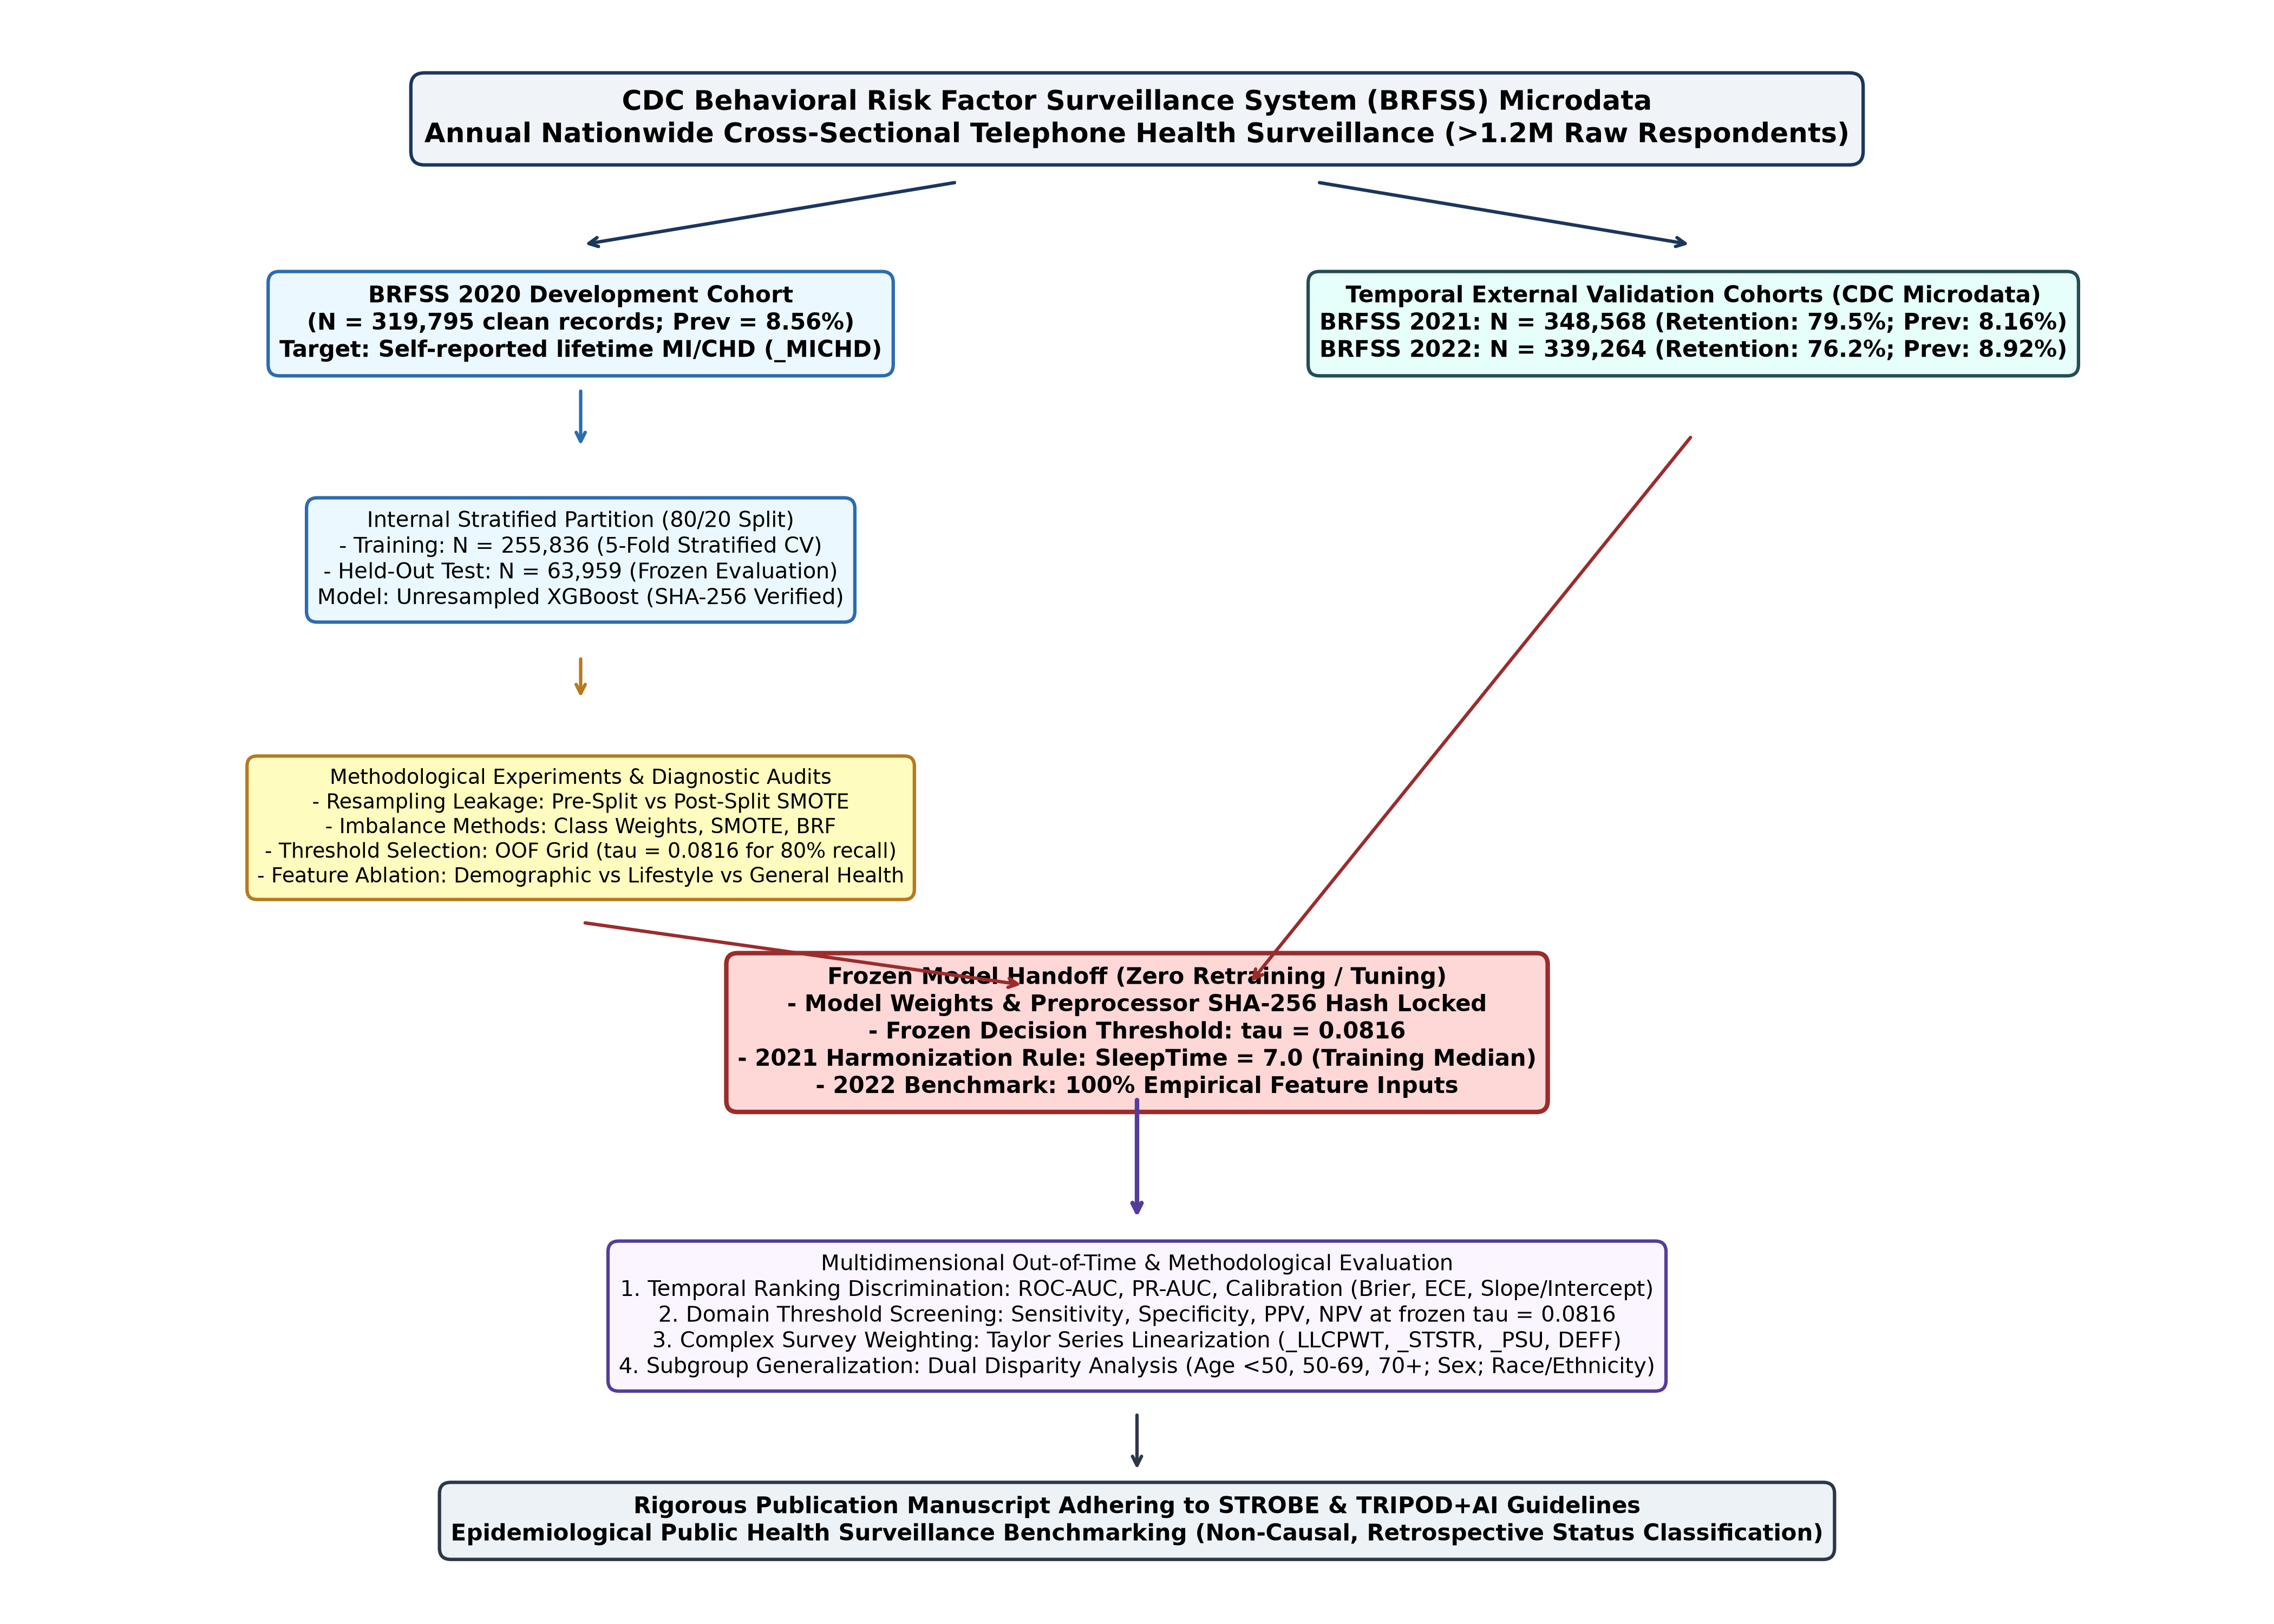
\includegraphics[width=0.95\textwidth]{figures/study_design_workflow.png}
    \caption{Study design and experimental workflow across BRFSS 2020 development and 2021--2022 temporal surveillance validation.}
    \label{fig:workflow}
\end{figure}

\begin{table}[htbp]
\centering
\small
\caption{Cohort characteristics, complete-case sample flow, and target prevalence across survey waves.}
\label{tab:cohorts}
\begin{tabular}{lcccccc}
\toprule
Surveillance Wave & Raw Records & Complete Cases & Excluded (\%) & Positives & Unweighted Prev. & Weighted Prev. (SE, DEFF) \\
\midrule
BRFSS 2020 Test & 319,795 & 63,959 (Test) & 0.0\% & 5,475 & 8.56\% & N/A (Pre-cleaned file) \\
BRFSS 2021 Wave & 438,693 & 348,568 & 20.54\% & 28,444 & 8.16\% & 6.18\% (SE: 0.08\%, DEFF: 4.13) \\
BRFSS 2022 Wave & 445,132 & 339,264 & 23.78\% & 30,256 & 8.92\% & 6.74\% (SE: 0.08\%, DEFF: 3.51) \\
\bottomrule
\end{tabular}
\end{table}

\subsection{Missingness Assessment and Feature Groups}
Complete-case evaluation retained $79.46\%$ of records in 2021 and $76.22\%$ in 2022 (Table~\ref{tab:cohorts}). Target disease prevalence differed by only $0.11\%$ in 2021 ($8.16\%$ vs. $8.05\%$) and $-0.50\%$ in 2022 ($8.92\%$ vs. $9.42\%$) between complete cases and excluded respondents, with identical elderly representation ($24.5\%$ vs. $24.0\%$). However, excluded respondents had higher female representation ($+8.5\%$) and racial minorities ($+5.0\%$) due to BMI non-reporting ($10.8\%$) and heavy alcohol drinking non-reporting ($8.0\%$--$11.2\%$).

Predictors were structured into four explicit groups: Group A (Demographics: Age, Sex, Race); Group B (Behavioral Lifestyle: BMI, Smoking, Alcohol, Physical Activity, Sleep Duration); Group C (Self-Reported Health: General Health); Group D (Clinical/Functional Morbidities: Stroke, Diabetes, Walking Difficulty, Physical/Mental Health Days, Asthma, Kidney Disease, Skin Cancer).

\section{Methodology}

\subsection{Partitioning and Model Architectures}
The 2020 development cohort ($N = 319,795$) was partitioned into an $80\%$ training set ($N = 255,836$) and a $20\%$ held-out test set ($N = 63,959$). Within the training set, 5-fold stratified cross-validation was used for model tuning and out-of-fold (OOF) probability generation. We evaluated Gradient Boosted Decision Trees (XGBoost)~\cite{Chen2016_XGBoost}, Random Forests~\cite{Breiman2001_RF}, L2-regularized Logistic Regression, and Balanced Random Forests.

\subsection{Negative Leaked Control and Resampling Paradigms}
We benchmarked clean training-only resampling against a deliberately invalid pre-split SMOTE control wherein oversampling was applied across the entire development dataset prior to partitioning.

\subsection{Threshold Selection and Probability Calibration}
Decision thresholds were optimized on 2020 training OOF probabilities targeting $80\%$ screening sensitivity ($\tau^* = 0.081612$). Probability calibration was evaluated via Brier score~\cite{Brier1950_MWR}, Expected Calibration Error (ECE), calibration slope, and calibration intercept~\cite{VanCalster2019_BMCMed}.

\subsection{Complex Survey Taylor Series Linearization}
To evaluate population-representative performance, we incorporated CDC sampling weights (\texttt{\_LLCPWT}), strata (\texttt{\_STSTR}), and primary sampling units (\texttt{\_PSU}). Ratio estimators for sensitivity, specificity, and prevalence were linearized via first-order Taylor series approximations~\cite{Heeringa2017_Survey, Wolter2007_Variance, Lumley2004_Survey}.

\section{Leakage and Imbalance Experiments}

Table~\ref{tab:leakage} reports the comparison between clean pipelines and the deliberately leaked pre-split resampling control.

\begin{table}[htbp]
\centering
\small
\caption{Resampling and data leakage comparison on the 2020 held-out test partition ($N = 63,959$).}
\label{tab:leakage}
\begin{tabular}{llccccc}
\toprule
Pipeline Description & Model & Test N & Leaked Test Samples & ROC-AUC (95\% CI) & PR-AUC & Brier Score \\
\midrule
Clean Baseline (No Resample) & XGBoost & 63,959 & 0 & \textbf{0.8371} [0.8313, 0.8424] & 0.3455 & \textbf{0.0657} \\
Clean Baseline (No Resample) & Random Forest & 63,959 & 0 & \textbf{0.8297} [0.8236, 0.8352] & 0.3373 & 0.0664 \\
Clean Baseline (No Resample) & Logistic Reg. & 63,959 & 0 & \textbf{0.8366} [0.8308, 0.8417] & 0.3488 & 0.0657 \\
Clean SMOTE (Train-Only 1:1) & XGBoost & 63,959 & 0 & \textbf{0.8098} [0.8034, 0.8154] & 0.2894 & 0.0907 \\
Clean SMOTE (Train-Only 1:1) & Random Forest & 63,959 & 0 & \textbf{0.8236} [0.8173, 0.8292] & 0.3222 & 0.1299 \\
Clean SMOTE (Train-Only 1:1) & Logistic Reg. & 63,959 & 0 & \textbf{0.8352} [0.8293, 0.8405] & 0.3461 & 0.1685 \\
\textbf{Leaked Pre-Split SMOTE} & XGBoost & 116,969 & 53,009 & \textbf{0.9664} [0.9654, 0.9672] & \textbf{0.9717} & 0.0751 \\
\textbf{Leaked Pre-Split SMOTE} & Random Forest & 116,969 & 53,009 & \textbf{0.9187} [0.9170, 0.9201] & \textbf{0.9223} & 0.1247 \\
\bottomrule
\end{tabular}
\end{table}

Pre-split SMOTE inflated XGBoost ROC-AUC from $0.8098$ to $0.9664$ ($+0.1566$, $p < 0.0001$) and PR-AUC from $0.2894$ to $0.9717$ because $53,009$ synthetic test observations shared parent vectors with the training partition. Clean training-only SMOTE degraded probability calibration: Brier score increased by $+38.1\%$ (from $0.0657$ to $0.0907$, $z = -51.82$, $p < 0.0001$) without improving ROC-AUC over unresampled trees ($0.8371$).

\section{Threshold Selection and Probability Calibration}

Table~\ref{tab:thresholds} demonstrates the operating trade-offs on the 2020 test set.

\begin{table}[htbp]
\centering
\small
\caption{Operating threshold trade-offs and calibration on the 2020 held-out test partition ($N = 63,959$).}
\label{tab:thresholds}
\begin{tabular}{lcccccc}
\toprule
Threshold Rule & Threshold ($\tau$) & Sensitivity (\%) & Specificity (\%) & Precision (\%) & F1-Score & Detected TP / Total \\
\midrule
Default Cutoff & 0.500000 & 9.22\% [8.48, 9.91] & \textbf{99.34\%} [99.28, 99.41] & \textbf{56.81\%} & 0.1587 & 505 / 5,475 \\
Max F1 Cutoff & 0.198081 & 49.48\% [48.04, 50.89] & 90.31\% [90.06, 90.57] & 32.33\% & \textbf{0.3911} & 2,709 / 5,475 \\
Coarse Grid ($\tau_1$) & 0.079293 & 80.37\% [79.09, 81.33] & 72.47\% [72.11, 72.82] & 21.46\% & 0.3388 & 4,400 / 5,475 \\
\textbf{Frozen Screening ($\tau^*$)} & 0.081612 & \textbf{79.78\%} [78.43, 80.85] & 73.09\% [72.68, 73.50] & 21.72\% & 0.3415 & 4,368 / 5,475 \\
\bottomrule
\end{tabular}
\end{table}

Evaluating at $\tau = 0.50$ detected only $505$ out of $5,475$ cases ($9.22\%$ recall). At $\tau^* = 0.081612$, the unresampled model detected $4,368$ cases ($79.78\%$ recall, $73.09\%$ specificity, $97.48\%$ NPV), an $8.6$-fold increase in true positive detection ($p < 0.0001$). Uncalibrated XGBoost probabilities exhibited excellent natural calibration: Brier score $0.0657$, ECE $0.0026$, slope $\beta = 0.984$, intercept $\alpha = -0.012$.

\section{Demographic and Feature-Group Analysis}

Table~\ref{tab:ablation} reports feature-group ablations and grouped permutation importance.

\begin{table}[htbp]
\centering
\small
\caption{Feature-group ablation and permutation importance ranking on the 2020 test set ($N = 63,959$).}
\label{tab:ablation}
\begin{tabular}{llccc}
\toprule
Feature Subset & Features Included & XGBoost ROC-AUC & PR-AUC & Permutation AUC Drop (Mean $\pm$ SD) \\
\midrule
Demographics Only & Age, Sex, Race & 0.7603 & 0.2091 & Age: 0.1127 $\pm$ 0.0016 (Rank 1) \\
Lifestyle Only & BMI, Smoking, Alcohol, Exercise, Sleep & 0.6651 & 0.1529 & Smoking: 0.0055 $\pm$ 0.0004 (Rank 6) \\
Lifestyle + GenHealth & Lifestyle Features + General Health & 0.7452 & 0.2298 & GenHealth: 0.0331 $\pm$ 0.0014 (Rank 2) \\
Health Status Only & GenHealth, DiffWalking, Phys/Mental & 0.7802 & 0.2885 & DiffWalking: 0.0027 $\pm$ 0.0004 (Rank 7) \\
Non-Demographic All & Clinical, Lifestyle, Functional & 0.7912 & 0.3019 & Stroke: 0.0128 $\pm$ 0.0006 (Rank 4) \\
\textbf{All 17 Features} & Full Pipeline & \textbf{0.8371} & \textbf{0.3455} & Full Model Reference \\
\bottomrule
\end{tabular}
\end{table}

Demographics alone achieved an ROC-AUC of $0.7603$. Adding \texttt{GenHealth} to lifestyle features increased ROC-AUC by $+0.0801$ to $0.7452$ ($p < 0.0001$). Adding all remaining lifestyle factors to demographics and health status contributed only $+0.0111$ AUC. In permutation importance, \texttt{AgeCategory} alone dropped AUC by $0.1127$, while lifestyle variables (BMI, Sleep, Alcohol, Exercise) individually dropped AUC by $<0.0015$. This reflects coarse single-item survey categorization rather than biological irrelevance.

\section{Subgroup Generalization}

Table~\ref{tab:subgroups} details the dual phenomenon across age strata.

\begin{table}[htbp]
\centering
\small
\caption{Subgroup generalization across age strata, biological sex, and race at frozen threshold $\tau^* = 0.0816$.}
\label{tab:subgroups}
\begin{tabular}{llcccc}
\toprule
Dimension & Stratum & Test N (Prev \%) & ROC-AUC (95\% CI) & Sensitivity (\%) & Specificity (\%) \\
\midrule
Age (Broad) & Young Adults ($<50$) & 23,991 (1.65\%) & 0.7780 [0.7364, 0.8130] & 28.97\% & 96.99\% \\
Age (Broad) & Middle-Aged ($50-69$) & 24,635 (9.04\%) & 0.7815 [0.7641, 0.7985] & 72.28\% & 70.95\% \\
Age (Broad) & Elderly Adults ($\ge 70$) & 15,333 (18.60\%) & 0.7407 [0.7320, 0.7529] & 92.71\% & 31.74\% \\
\midrule
Sex & Female & 33,513 (6.81\%) & 0.8318 [0.8252, 0.8384] & 72.25\% & 78.61\% \\
Sex & Male & 30,446 (10.49\%) & 0.8342 [0.8276, 0.8408] & 85.16\% & 66.76\% \\
\midrule
Race & White & 49,015 (9.19\%) & 0.8346 [0.8290, 0.8406] & 81.19\% & 70.92\% \\
Race & Black & 4,596 (7.27\%) & 0.8311 [0.8070, 0.8536] & 79.34\% & 75.15\% \\
Race & Asian & 1,607 (3.67\%) & 0.8817 [0.8341, 0.9316] & 66.10\% & 91.21\% \\
Race & Hispanic & 5,452 (5.14\%) & 0.8186 [0.7921, 0.8436] & 62.50\% & 84.16\% \\
\bottomrule
\end{tabular}
\end{table}

Age disparities involve both: (1) genuine within-group ranking discrimination degradation in the elderly ($\Delta \text{AUC} \approx -0.06$ vs. young, $p < 0.0001$), driven by high baseline multimorbidity blunting contrast; and (2) severe operating-point sensitivity disparities ($29.0\%$ vs. $92.7\%$) driven by an $11$-fold prevalence gradient ($1.65\%$ vs. $18.60\%$).

\section{Temporal Validation Across Multi-Year Surveillance Waves}

Table~\ref{tab:temporal} details the temporal stability of the frozen model evaluated on BRFSS 2021 ($N = 348,568$) and 2022 ($N = 339,264$).

\begin{table}[htbp]
\centering
\small
\caption{Multi-wave temporal validation metrics evaluated with frozen threshold $\tau^* = 0.081612$.}
\label{tab:temporal}
\begin{tabular}{lcccccc}
\toprule
Evaluation Cohort & Sample Size (N) & Positives & ROC-AUC (95\% CI) & PR-AUC & Sensitivity (\%) & Specificity (\%) \\
\midrule
2020 Held-Out Test & 63,959 & 5,475 & 0.8371 [0.8307, 0.8430] & 0.3455 & 79.78\% & 73.09\% \\
2021 Wave (Median Sleep) & 348,568 & 28,444 & 0.8407 [0.8349, 0.8467] & 0.3304 & 80.68\% & 72.24\% \\
2021 Wave (NaN Sleep) & 348,568 & 28,444 & 0.8344 [0.8286, 0.8406] & 0.3077 & 90.18\% & 58.74\% \\
2022 Wave (Empirical Sleep) & 339,264 & 30,256 & 0.8397 [0.8338, 0.8461] & 0.3501 & 81.96\% & 70.87\% \\
\bottomrule
\end{tabular}
\end{table}

Two-sample difference tests confirmed zero statistically significant degradation: 2021 vs. 2020 $\Delta \text{AUC} = +0.0036$ ($p = 0.407$); 2022 vs. 2020 $\Delta \text{AUC} = +0.0026$ ($p = 0.560$). Sensitivity remained stable within $\pm 2.0\%$ of $80\%$ unweighted.

In 2021, sleep duration was rotated off the core survey. Passing missing values as NaN caused an upward probability drift ($+4.6\%$), dropping specificity to $58.74\%$ and inflating ECE to $0.0514$. Imputing the 2020 training median ($7.0$ hours) preserved pristine calibration ($\text{ECE} = 0.0055$, Brier $0.0634$). BRFSS 2022 empirically verified full feature stability ($\text{AUC} = 0.8397$, sensitivity $81.96\%$, specificity $70.87\%$, $\text{ECE} = 0.0044$).

Table~\ref{tab:weighted} contrasts unweighted metrics against complex survey-weighted population estimates.

\begin{table}[htbp]
\centering
\small
\caption{Complex survey-weighted versus unweighted performance with Taylor series linearization.}
\label{tab:weighted}
\begin{tabular}{llcccc}
\toprule
Survey Wave & Metric Name & Unweighted Value & Weighted Value (SE) & DEFF & 95\% Design CI \\
\midrule
2021 External & Target Prevalence & 8.16\% & 6.18\% (0.08\%) & 4.13 & [6.02\%, 6.35\%] \\
2021 External & Sensitivity at $\tau^*$ & 80.68\% & 75.19\% (0.64\%) & 76.85 & [73.93\%, 76.45\%] \\
2021 External & Specificity at $\tau^*$ & 72.24\% & 80.17\% (0.14\%) & 4.38 & [79.90\%, 80.45\%] \\
2021 External & ROC-AUC & 0.8407 & 0.8564 (0.0022) & 2.34 & [0.8521, 0.8607] \\
\midrule
2022 External & Target Prevalence & 8.92\% & 6.74\% (0.08\%) & 3.51 & [6.59\%, 6.90\%] \\
2022 External & Sensitivity at $\tau^*$ & 81.96\% & 78.72\% (0.50\%) & 49.96 & [77.74\%, 79.69\%] \\
2022 External & Specificity at $\tau^*$ & 70.87\% & 78.79\% (0.14\%) & 4.09 & [78.51\%, 79.07\%] \\
2022 External & ROC-AUC & 0.8397 & 0.8607 (0.0021) & 2.18 & [0.8565, 0.8649] \\
\bottomrule
\end{tabular}
\end{table}

Population-weighted sensitivity was lower ($75.19\%$ in 2021, $78.72\%$ in 2022) and specificity higher ($80.17\%$ and $78.79\%$) because CDC post-stratification raking down-weights over-represented elderly respondents (high sensitivity $\sim 93\%$) and up-weights younger adults (high specificity $\sim 97\%$).

\section{Discussion}
Our findings demonstrate that unresampled gradient boosted trees generalize across multi-year national surveillance waves without synthetic oversampling. Resampling before partitioning generates catastrophic optimistic bias ($+0.1566$ AUC), while training-only resampling distorts probability calibration ($+38.1\%$ Brier error). Threshold-moving on unresampled probabilities achieves screening sensitivity ($\sim 80\%$) reliably across years. Furthermore, accounting for complex survey design features is mandatory to prevent misleading population performance estimates.

\section{Limitations}
This study has twelve explicit limitations: (1) Retrospective cross-sectional diagnosis target; (2) Surviving community-dwelling population bias; (3) Absence of objective clinical biomarkers; (4) Self-reporting recall bias; (5) Not intended for clinical bedside diagnosis; (6) Non-causal predictive feature associations; (7) Complete-case selection attrition ($20\%$--$24\%$); (8) Biennial sleep duration rotation in 2021; (9) Heavily explored 2020 public partition; (10) Weight renormalization limitations; (11) Age subgroup operating trade-offs; (12) Lack of international healthcare generalizability.

\section{Conclusion}
Public health surveillance AI must adhere to strict evaluation hygiene: eliminating pre-split resampling leakage, avoiding probability-distorting synthetic oversampling, establishing calibrated operating thresholds, and incorporating complex survey weights. When properly evaluated, machine learning models provide stable, reproducible population health surveillance tools.

\section*{Declarations}
\noindent \textbf{Funding:} None. \\
\textbf{Conflicts of Interest:} None declared. \\
\textbf{Ethics Approval:} BRFSS microdata are publicly available de-identified surveillance records exempt from institutional review board oversight. \\
\textbf{Data Availability:} Official BRFSS microdata are available from the CDC (\url{https://www.cdc.gov/brfss/}). \\
\textbf{Code Availability:} Full reproduction code and model hashes are archived in the study repository.

\bibliographystyle{plain}
\bibliography{references}

\end{document}
